
\providecommand{\Cat}{\mathcal{C}at}
\providecommand{\sSet}{s\mathcal{S}et}

\section{富集\trNaturalTransformation{}与富集\trYonedaLemma}\label{sec:enriched-yoneda-lemma}

回忆：平行\trFunctor{} $F,G\colon\mathcal{C}\to\mathcal{D}$ 之间的一个（非富集的）%
\trNaturalTransformation{} $\alpha\colon F\Rightarrow G$ 由下列数据给出：
\begin{itemize}
\item 对每个 $x\in\mathcal{C}$，一条箭头 $\alpha_{x}\in\mathcal{D}(Fx,Gx)$ 的
  数据；
\item 并要求对每个态射 $f\in\mathcal{C}(x,y)$，图表
\begin{rveq}\label{eq:unenriched-naturality-square}
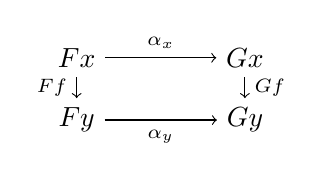
\begin{tikzpicture}[x=1.9em,y=1.5em]
  \node (tl) at (0,1.5) {$Fx$};
  \node (tr) at (3.2,1.5) {$Gx$};
  \node (bl) at (0,0) {$Fy$};
  \node (br) at (3.2,0) {$Gy$};
  \draw[->] (tl) -- node[above]{$\scriptstyle\alpha_{x}$} (tr);
  \draw[->] (tl) -- node[left]{$\scriptstyle Ff$} (bl);
  \draw[->] (tr) -- node[right]{$\scriptstyle Gf$} (br);
  \draw[->] (bl) -- node[below]{$\scriptstyle\alpha_{y}$} (br);
\end{tikzpicture}
\end{rveq}
  在 $\mathcal{D}$ 中交换。
\end{itemize}

这一概念可富集为 $\mathcal{V}$-\trNaturalTransformation{}的概念：其数据恰好
相同——即 $\mathcal{D}$ 的底\trCategory{}中由 $\mathcal{C}$ 的诸对象加标的一族
箭头——但带有一个更强的 $\mathcal{V}$-自然性条件，后者经由把自然性条件
\eqref{eq:unenriched-naturality-square} 内化而得到表达。

\begin{definition}\label{def:vnatural-transformation}
介于 $\mathcal{V}$-富集\trFunctor{} $F,G\colon\mathcal{C}\to\mathcal{D}$ 之间的
$\mathcal{V}$\textbf{-富集\trNaturalTransformation}（$\mathcal{V}$-enriched
natural transformation）或称 $\mathcal{V}$\textbf{-\trNaturalTransformation}
（$\mathcal{V}$-natural transformation）$\alpha\colon F\Rightarrow G$ 由下列
数据给出：
\begin{itemize}
\item 对每个 $x\in\mathcal{C}$，一条箭头 $\alpha_{x}\colon 1\to\mathcal{D}(Fx,Gx)$；
\item 使得对每一对对象 $x$，$y\in\mathcal{C}$，下述 $\mathcal{V}$-自然性方块在
  $\mathcal{V}$ 中交换：
\begin{rveq}\label{eq:vnaturality-square}
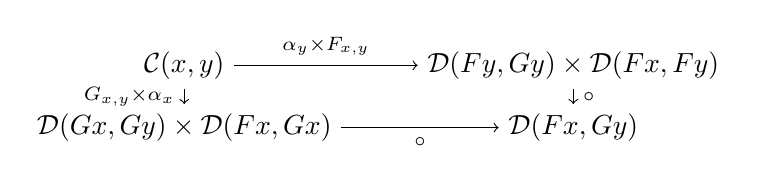
\begin{tikzpicture}[x=1.9em,y=1.5em]
  \node (tl) at (0,1.5) {$\mathcal{C}(x,y)$};
  \node (tr) at (7.4,1.5) {$\mathcal{D}(Fy,Gy)\times\mathcal{D}(Fx,Fy)$};
  \node (bl) at (0,0) {$\mathcal{D}(Gx,Gy)\times\mathcal{D}(Fx,Gx)$};
  \node (br) at (7.4,0) {$\mathcal{D}(Fx,Gy)$};
  \draw[->] (tl) -- node[above]{$\scriptstyle\alpha_{y}\times F_{x,y}$} (tr);
  \draw[->] (tl) -- node[left]{$\scriptstyle G_{x,y}\times\alpha_{x}$} (bl);
  \draw[->] (tr) -- node[right]{$\scriptstyle\circ$} (br);
  \draw[->] (bl) -- node[below]{$\scriptstyle\circ$} (br);
\end{tikzpicture}
\end{rveq}
\end{itemize}
\end{definition}

\begin{example}\label{exa:post-composition-vnatural-transformation}
一个 $\mathcal{V}$-\trCategory{} $\mathcal{C}$ 的底\trCategory{}中的一条箭头
$f\colon 1\to\mathcal{C}(x,y)$ 定义一支 $\mathcal{V}$-\trNaturalTransformation
$-\circ f\colon\mathcal{C}(y,-)\Rightarrow\mathcal{C}(x,-)$——介于诸富集可表示%
\trFunctor{}之间——其在 $z\in\mathcal{C}$ 处的分量由在 $f$ 处对复合映射的伴随转置
求值而定义：
\[ 1\xrightarrow{\ f\ }\mathcal{C}(x,y)
   \xrightarrow{\ \mathcal{C}(-,z)_{x,y}\ }\mathcal{C}(x,z)^{\mathcal{C}(y,z)} \]
所要求的 $\mathcal{V}$-自然性方块，经由对 $\mathcal{C}$ 的结合律图表求一个分量
之值而得到。
\end{example}

$\mathcal{V}$-\trNaturalTransformation{}的复合方式与非富集的%
\trNaturalTransformation{}相同：

\begin{definition}\label{def:vertical-horizontal-composites}
介于 $\mathcal{C}$ 与 $\mathcal{D}$ 之间的 $\mathcal{V}$-\trNaturalTransformation
$\alpha\colon F\Rightarrow G$ 与 $\beta\colon G\Rightarrow H$ 的\textbf{竖直复合}
（vertical composite）$\beta\cdot\alpha$ 在 $x\in\mathcal{C}$ 处的分量
$(\beta\cdot\alpha)_{x}$ 定义为复合
\[ 1\xrightarrow{\ \beta_{x}\times\alpha_{x}\ }
   \mathcal{D}(Gx,Hx)\times\mathcal{D}(Fx,Gx)
   \xrightarrow{\ \circ\ }\mathcal{D}(Fx,Hx) \]
从 $\mathcal{C}$ 到 $\mathcal{D}$ 的 $\alpha\colon F\Rightarrow G$ 与从
$\mathcal{D}$ 到 $\mathcal{E}$ 的 $\gamma\colon H\Rightarrow K$ 的\textbf{水平
复合}（horizontal composite）$\gamma*\alpha$ 在 $x\in\mathcal{C}$ 处的分量
$(\gamma*\alpha)_{x}$ 定义为公共复合
\begin{center}
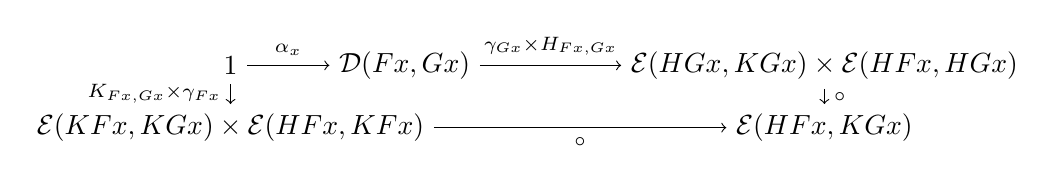
\begin{tikzpicture}[x=1.85em,y=1.5em]
  \node (tl) at (0,1.5) {$1$};
  \node (tm) at (3.4,1.5) {$\mathcal{D}(Fx,Gx)$};
  \node (tr) at (11.6,1.5) {$\mathcal{E}(HGx,KGx)\times\mathcal{E}(HFx,HGx)$};
  \node (bl) at (0,0) {$\mathcal{E}(KFx,KGx)\times\mathcal{E}(HFx,KFx)$};
  \node (br) at (11.6,0) {$\mathcal{E}(HFx,KGx)$};
  \draw[->] (tl) -- node[above]{$\scriptstyle\alpha_{x}$} (tm);
  \draw[->] (tm) -- node[above]{$\scriptstyle\gamma_{Gx}\times H_{Fx,Gx}$} (tr);
  \draw[->] (tl) -- node[left]{$\scriptstyle K_{Fx,Gx}\times\gamma_{Fx}$} (bl);
  \draw[->] (tr) -- node[right]{$\scriptstyle\circ$} (br);
  \draw[->] (bl) -- node[below]{$\scriptstyle\circ$} (br);
\end{tikzpicture}
\end{center}
它由 $\gamma$ 的 $\mathcal{V}$-自然性给出良定义。\footnote{原书此图右上节点
印作「$\mathcal{E}(KGx,HGx)\times\mathcal{E}(HFx,HGx)$」，按公共复合之型两
因子次序倒置；右下节点花体印作「$\mathcal{D}(HFx,KGx)$」，$\mathcal{D}$ 疑为
$\mathcal{E}$ 之误；均径改。——译者注}这些构造的 $\mathcal{V}$-自然性
留作\cref{ex:vertical-horizontal-vnatural}。
\end{definition}

一支 $\mathcal{V}$-\trNaturalTransformation{}的\textbf{底自然变换}（underlying
natural transformation）由同一族箭头给出。非富集的自然性条件
\eqref{eq:unenriched-naturality-square} 经由在一条底箭头
$f\colon 1\to\mathcal{C}(x,y)$ 处对富集自然性条件
\eqref{eq:vnaturality-square} 求值而得到。特别地，$\mathcal{V}$-%
\trNaturalTransformation{}的竖直复合与水平复合的中间四项交换规则（见附录 B 中的%
\cref{def:two-category}）由非富集\trNaturalTransformation{}的竖直复合与水平复合的中间四项交换
规则推得，盖因后者的数据决定前者的数据。从而，%
\cref{ex:vertical-horizontal-vnatural} 蕴含：

\begin{corollary}\label{cor:vcat-two-category}
对任何\trCartesianClosed{}\trCategory{} $\mathcal{V}$，存在一个由 $\mathcal{V}$-%
\trCategory、$\mathcal{V}$-\trFunctor{}与 $\mathcal{V}$-\trNaturalTransformation{}%
组成的 2-\trCategory{} $\mathcal{V}\text{-}\Cat$。
\end{corollary}

我们如今将注意力转向 $\mathcal{V}$-富集\trYonedaLemma，我们将以若干形式陈述之。
\trYonedaLemma{}的一个角色，是给出 $\mathcal{C}$ 中同构对象的一个可表示刻画。当
$\mathcal{C}$ 是一个 $\mathcal{V}$-\trCategory{}时，这有若干形式。下述结果中所
谈及的 $\mathcal{V}$\textbf{-自然同构}（$\mathcal{V}$-natural isomorphism）
概念，定义为一支带有关于竖直复合之逆 $\alpha^{-1}\colon G\Rightarrow F$ 的
$\mathcal{V}$-\trNaturalTransformation{} $\alpha\colon F\Rightarrow G$。

\begin{lemma}\label{lem:isomorphism-characterizations}
对 $\mathcal{V}$-\trCategory{} $\mathcal{C}$ 中的对象 $x$ 与 $y$，下述诸款等价：
\begin{enumerate}[label=(\roman*)]
\item $x$ 与 $y$ 作为 $\mathcal{C}$ 的底\trCategory{}的对象是同构的。
\item 取值于 $\mathcal{S}et$ 的诸非富集可表示函子
  $\mathcal{C}(x,-),\mathcal{C}(y,-)\colon\mathcal{C}\to\mathcal{S}et$ 是自然
  同构的。
\item 取值于 $\mathcal{V}$ 的诸非富集可表示函子
  $\mathcal{C}(x,-),\mathcal{C}(y,-)\colon\mathcal{C}\to\mathcal{V}$ 是自然
  同构的。
\item 取值于 $\mathcal{V}$ 的诸 $\mathcal{V}$-\trFunctor{}
  $\mathcal{C}(x,-),\mathcal{C}(y,-)\colon\mathcal{C}\to\mathcal{V}$ 是
  $\mathcal{V}$-自然同构的。
\end{enumerate}
\end{lemma}

\begin{proof}
应用底范畴 2-\trFunctor{} $(-)_{0}\colon\mathcal{V}\text{-}\Cat\to\Cat$，第四款
蕴含第三款。第三款经由与底集函子 $(-)_{0}\colon\mathcal{V}\to\mathcal{S}et$ 作%
\trWhiskering{}而蕴含第二款。第二款由非富集的\trYonedaLemma{}蕴含第一款；这仍是
要点所在。最后，第一款经由一个直接构造蕴含第四款：若
$f\colon 1\to\mathcal{C}(x,y)$ 与 $g\colon 1\to\mathcal{C}(y,x)$ 在 $\mathcal{C}$
的底\trCategory{}中定义一个\trIsomorphism，则%
\cref{exa:post-composition-vnatural-transformation}中相应的可表示
$\mathcal{V}$-\trNaturalTransformation{}定义一个 $\mathcal{V}$-自然同构。
\end{proof}

\cref{lem:isomorphism-characterizations}定义了富集\trCategory{}的两对象之间的一个
常见的\textbf{\trIsomorphism}概念，而这一概念最终与通常非富集的同构概念并无
不同。这可以视为定义了富集\trYonedaLemma{}的一种「廉价」形式。$\mathcal{V}$-%
\trYonedaLemma{}的完全形式将通常的陈述——介于「定义域为一支可表示\trFunctor{}的
那些\trNaturalTransformation{}所成之集」与「由在表示对象处对陪域求值所定义之集」
之间的一个自然\trIsomorphism——富集为 $\mathcal{V}$ 中的一个\trIsomorphism。
使之精确的第一步，是将一对平行 $\mathcal{V}$-\trFunctor{}之间的
$\mathcal{V}$-\trNaturalTransformation{}之集富集为 $\mathcal{V}$ 的一个对象。

\begin{definition}\label{def:vobject-natural-transformations}
设 $\mathcal{V}$ 是一个\trComplete{}\trCartesianClosed{}\trCategory，并考虑
$\mathcal{V}$-\trFunctor{}的一个平行对 $F,G\colon\mathcal{C}\to\mathcal{D}$，其中
$\mathcal{C}$ 是一个小 $\mathcal{V}$-\trCategory。于是，
$\mathcal{V}$\textbf{-\trNaturalTransformation{}对象}（$\mathcal{V}$-object of
$\mathcal{V}$-natural transformations）由等化子图表（equalizer diagram）
\[ \mathcal{D}^{\mathcal{C}}(F,G)\longrightarrow
   \prod_{z\in\mathcal{C}}\mathcal{D}(Fz,Gz)
   \;\rightrightarrows\;
   \prod_{x,y\in\mathcal{C}}\mathcal{D}(Fx,Gy)^{\mathcal{C}(x,y)} \]
定义，其中等化子图表中指向 $\mathcal{D}(Fx,Gy)^{\mathcal{C}(x,y)}$ 的两个映射，
一个由投射到 $\mathcal{D}(Fx,Gx)$、施加 $G$ 在箭头上的内部作用（internal
action）、然后再复合而定义，另一个则由投射到 $\mathcal{D}(Fy,Gy)$、施加 $F$ 在
箭头上的内部作用、然后再复合而定义：
\begin{center}
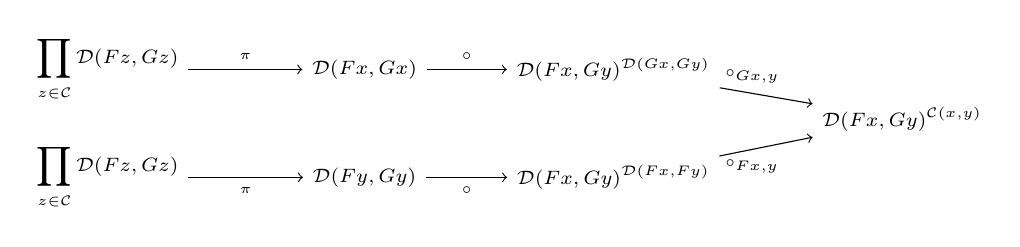
\begin{tikzpicture}[x=1.45em,y=1.5em,every node/.style={font=\scriptsize}]
  \node (pl) at (0,1.5) {$\displaystyle\prod_{z\in\mathcal{C}}\mathcal{D}(Fz,Gz)$};
  \node (t1) at (6.4,1.5) {$\mathcal{D}(Fx,Gx)$};
  \node (t2) at (12.6,1.5) {$\mathcal{D}(Fx,Gy)^{\mathcal{D}(Gx,Gy)}$};
  \node (r)  at (19.8,0.3) {$\mathcal{D}(Fx,Gy)^{\mathcal{C}(x,y)}$};
  \node (bl) at (0,-1.1) {$\displaystyle\prod_{z\in\mathcal{C}}\mathcal{D}(Fz,Gz)$};
  \node (b1) at (6.4,-1.1) {$\mathcal{D}(Fy,Gy)$};
  \node (b2) at (12.6,-1.1) {$\mathcal{D}(Fx,Gy)^{\mathcal{D}(Fx,Fy)}$};
  \draw[->] (pl) -- node[above]{$\scriptstyle\pi$} (t1);
  \draw[->] (t1) -- node[above]{$\scriptstyle\circ$} (t2);
  \draw[->] (t2) -- node[above,pos=0.35]{$\scriptstyle\circ_{Gx,y}$} (r);
  \draw[->] (bl) -- node[below]{$\scriptstyle\pi$} (b1);
  \draw[->] (b1) -- node[below]{$\scriptstyle\circ$} (b2);
  \draw[->] (b2) -- node[below,pos=0.35]{$\scriptstyle\circ_{Fx,y}$} (r);
\end{tikzpicture}
\end{center}
\end{definition}

\begin{lemma}\label{lem:underlying-set-of-vobject}
$\mathcal{V}$-\trNaturalTransformation{}对象
$\mathcal{V}^{\mathcal{C}}(F,G)$ 的底集，是从 $F$ 到 $G$ 的
$\mathcal{V}$-\trNaturalTransformation{}之集。
\end{lemma}

\begin{proof}
由其定义性的\trUniversalProperty，$\mathcal{V}^{\mathcal{C}}(F,G)$ 底集的诸%
\trElement{}对应于使\cref{def:vobject-natural-transformations}所述的平行映射对
等化的那些映射 $\alpha\colon 1\to\prod_{z\in\mathcal{C}}\mathcal{V}(Fz,Gz)$。
该映射 $\alpha$ 定义一支 $\mathcal{V}$-\trNaturalTransformation{}
$\alpha\colon F\Rightarrow G$ 的诸分量，而交换性条件转置后恰为
\eqref{eq:vnaturality-square}。
\end{proof}

\trYonedaLemma{}可以由「在恒同处求值是一个同构」这句口号来表达；但由于在富集情境
中，\trNaturalTransformation{}的富集对象是经由一个\trLimit{}定义的，较为容易的
做法是转而定义诱导出\trNaturalTransformation{}的那个映射。给定小
$\mathcal{V}$-\trCategory{} $\mathcal{A}$ 中的一个对象 $a\in\mathcal{A}$ 与一支
$\mathcal{V}$-\trFunctor{} $F\colon\mathcal{A}\to\mathcal{V}$，$F$ 在箭头上的内部
作用经转置而定义一个使平行对
\begin{rveq}\label{eq:internal-action-parallel-pair}
Fa\overset{F_{a,-}}{\dashrightarrow}\prod_{z\in\mathcal{A}}Fz^{\mathcal{A}(a,z)}
\;\rightrightarrows\;
\prod_{x,y\in\mathcal{A}}Fy^{\mathcal{A}(a,x)\times\mathcal{A}(x,y)}
\end{rveq}
等化的映射，从而在 $\mathcal{V}$ 中诱导一个典范映射
$Fa\to\mathcal{V}^{\mathcal{A}}(\mathcal{A}(a,-),F)$。

\begin{theorem}[富集\trYonedaLemma]\label{thm:enriched-yoneda}
对任何小 $\mathcal{V}$-\trCategory{} $\mathcal{A}$、对象 $a\in\mathcal{A}$ 与一支
$\mathcal{V}$-\trFunctor{} $F\colon\mathcal{A}\to\mathcal{V}$，该典范映射定义
$\mathcal{V}$ 中的一个\trIsomorphism
\[ Fa\simeq\mathcal{V}^{\mathcal{A}}(\mathcal{A}(a,-),F) \]
且该\trIsomorphism{}在 $a$ 与 $F$ 二者中都是 $\mathcal{V}$-自然的。
\end{theorem}

\begin{proof}
为证该\trIsomorphism，只需验证 \eqref{eq:internal-action-parallel-pair} 是一个%
\trLimit{}锥。为此，考虑该平行对上的另一个锥
\[ \nu\xrightarrow{\ \lambda\ }\prod_{z\in\mathcal{A}}Fz^{\mathcal{A}(a,z)}
   \;\rightrightarrows\;
   \prod_{x,y\in\mathcal{A}}Fy^{\mathcal{A}(a,x)\times\mathcal{A}(x,y)} \]
并经由在 $\mathrm{id}_{a}$ 处对分量 $\lambda_{a}$ 的转置求值而定义一个候选的因子
分解：
\[ \lambda_{a}(\mathrm{id}_{a})\coloneqq\nu
   \xrightarrow{\ \mathrm{id}_{a}\times\nu\ }\mathcal{A}(a,a)\times\nu
   \xrightarrow{\ \lambda_{a}\ }Fa \]
为证 $\lambda_{a}(\mathrm{id}_{a})\colon\nu\to Fa$ 确实定义 $\lambda$ 穿过该%
\trLimit{}锥的一个因子分解，只需在该乘积的每个分量 $Fz^{\mathcal{A}(a,z)}$ 处
证明交换性，我们以转置的形式验证之：
\begin{center}
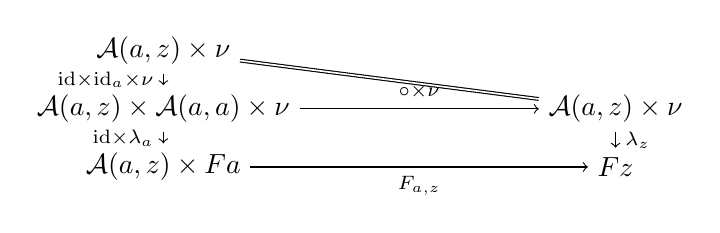
\begin{tikzpicture}[x=1.9em,y=1.4em]
  \node (t)  at (0,3.0) {$\mathcal{A}(a,z)\times\nu$};
  \node (ml) at (0,1.5) {$\mathcal{A}(a,z)\times\mathcal{A}(a,a)\times\nu$};
  \node (mr) at (8.6,1.5) {$\mathcal{A}(a,z)\times\nu$};
  \node (bl) at (0,0) {$\mathcal{A}(a,z)\times Fa$};
  \node (br) at (8.6,0) {$Fz$};
  \draw[->] (t) -- node[left]{$\scriptstyle\mathrm{id}\times\mathrm{id}_{a}\times\nu$} (ml);
  \draw[double] (t) -- (mr);
  \draw[->] (ml) -- node[above]{$\scriptstyle\circ\times\nu$} (mr);
  \draw[->] (ml) -- node[left]{$\scriptstyle\mathrm{id}\times\lambda_{a}$} (bl);
  \draw[->] (mr) -- node[right]{$\scriptstyle\lambda_{z}$} (br);
  \draw[->] (bl) -- node[below]{$\scriptstyle F_{a,z}$} (br);
\end{tikzpicture}
\end{center}
上方三角形由 $\mathcal{A}$ 的恒等律而交换，而下方方块之所以交换，是因为
$\lambda$ 定义平行对上的一个锥。因子分解 $\lambda_{a}(\mathrm{id}_{a})$ 的唯一
性由同一图表沿 $z=a$ 取值并在 $\mathrm{id}_{a}$ 处求值而推得。
$Fa\cong\mathcal{V}^{\mathcal{A}}(\mathcal{A}(a,-),F)$ 之 $\mathcal{V}$-自然性的
验证留给读者，或见文献 \cite[\S 2.4]{bib68}。
\end{proof}

过渡到底集：

\begin{corollary}\label{cor:yoneda-bijection}
对任何小 $\mathcal{V}$-\trCategory{} $\mathcal{A}$、对象 $a\in\mathcal{A}$ 与一支
$\mathcal{V}$-\trFunctor{} $F\colon\mathcal{A}\to\mathcal{V}$，在
$\mathcal{V}$-\trNaturalTransformation{} $\alpha\colon\mathcal{A}(a,-)\Rightarrow F$
与 $Fa$ 的底集中的诸\trElement{} $u\colon 1\to Fa$ 之间存在一个自然双射，后者由在
$a\in\mathcal{A}$ 处的分量于恒同 $\mathrm{id}_{a}$ 处求值而实现。
\end{corollary}

这就给出了一个证成 $\mathcal{V}$-\trFunctor{}之可表示性的判据：呈现确立定义性
$\mathcal{V}$-自然同构所需的最小数据即可。

\begin{corollary}\label{cor:represent-functor}
对一支 $\mathcal{V}$-\trFunctor{}
$F\colon\mathcal{A}^{\mathrm{op}}\to\mathcal{V}$ 与一个对象 $a\in\mathcal{A}$，
下述诸款等价，且它们定义「$a$ \textbf{表示}（represent）$F$」之所指：
\begin{enumerate}[label=(\roman*)]
\item 存在 $\mathcal{V}$ 中的一个\trIsomorphism{} $\mathcal{A}(x,a)\cong Fx$，
  其在 $x\in\mathcal{A}$ 中是 $\mathcal{V}$-自然的。
\item 存在 $Fa$ 的底集中的一个\trElement{} $u\colon 1\to Fa$，使得复合映射
\[ \mathcal{A}(x,a)\xrightarrow{\ F_{x,a}\ }\mathcal{V}(Fa,Fx)
   \xrightarrow{\ \circ u\ }\mathcal{V}(1,Fx)\cong Fx \]
  对一切 $x\in\mathcal{A}$ 都定义 $\mathcal{V}$ 中的一个\trIsomorphism。
\end{enumerate}
\end{corollary}

\begin{proof}
由\cref{cor:yoneda-bijection}，$Fa$ 底集中的\trElement{} $u\colon 1\to Fa$ 决定
一支唯一的 $\mathcal{V}$-\trNaturalTransformation{}
$\mathcal{A}(-,a)\Rightarrow F$，其在 $x\in\mathcal{A}$ 处的分量即陈述中的那个
映射。于是，泛\trElement{} $u$ 定义一个 $\mathcal{V}$-自然同构而不只是一支
$\mathcal{V}$-\trNaturalTransformation，恰当陈述中的那个映射是\trIsomorphism{}%
之时。
\end{proof}

既然我们已经假定富集之基是\trCartesianClosed，2-\trCategory{}
$\mathcal{V}\text{-}\Cat$ 便容许有限\trProduct，这使得我们能够定义多变量
$\mathcal{V}$-\trFunctor（见\cref{ex:v-bifunctor}）。下述结果蕴含：在 A.4 节与 A.5 节中由
$\mathcal{V}$-自然同构所刻画的那些结构可以拼装成 $\mathcal{V}$-\trFunctor。

\begin{proposition}\label{prop:unique-extension-vfunctor}
设 $M\colon\mathcal{B}^{\mathrm{op}}\times\mathcal{A}\to\mathcal{V}$ 是一支
$\mathcal{V}$-\trFunctor，使得对每个 $a\in\mathcal{A}$，$\mathcal{V}$-%
\trFunctor{} $M(-,a)\colon\mathcal{B}^{\mathrm{op}}\to\mathcal{V}$ 被某个
$Fa\in\mathcal{B}$ 所表示，意即存在一个 $\mathcal{V}$-自然\trIsomorphism
\[ \mathcal{B}(b,Fa)\cong M(b,a). \]
那么，存在唯一的方式把映射 $a\in\mathcal{A}\mapsto Fa\in\mathcal{B}$ 扩张为一支
$\mathcal{V}$-\trFunctor{} $F\colon\mathcal{A}\to\mathcal{B}$，使得诸%
\trIsomorphism{}在 $a\in\mathcal{A}$ 中以及在 $b\in\mathcal{B}$ 中都是
$\mathcal{V}$-自然的。
\end{proposition}

\begin{proof}
由\cref{cor:yoneda-bijection}之形式的\trYonedaLemma，对每个 $a\in\mathcal{A}$
定义一族在 $b\in\mathcal{B}$ 中 $\mathcal{V}$-自然的\trIsomorphism{}
$\alpha_{b,a}\colon\mathcal{B}(b,Fa)\cong M(b,a)$，就等于对每个
$a\in\mathcal{A}$ 定义一族满足\cref{cor:represent-functor}(ii)之条件的%
\trElement{} $\eta_{a}\colon 1\to M(Fa,a)$。由\trYonedaLemma{}中的
$\mathcal{V}$-自然性陈述，\trIsomorphism{} $\alpha_{b,a}$ 在 $a$ 中为
$\mathcal{V}$-自然，等价于\trElement{}之族 $\eta_{a}\colon 1\to M(Fa,a)$ 在 $a$
中「超自然地」$\mathcal{V}$-自然。这意味着：对任何一对对象
$a$，$a'\in\mathcal{A}$，外侧方块交换：
\begin{center}
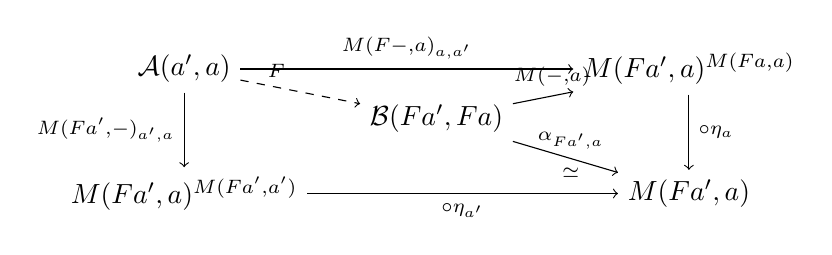
\begin{tikzpicture}[x=1.9em,y=1.5em]
  \node (tl) at (0,3.0) {$\mathcal{A}(a',a)$};
  \node (tr) at (9.6,3.0) {$M(Fa',a)^{M(Fa,a)}$};
  \node (c)  at (4.8,1.8) {$\mathcal{B}(Fa',Fa)$};
  \node (bl) at (0,0) {$M(Fa',a)^{M(Fa',a')}$};
  \node (br) at (9.6,0) {$M(Fa',a)$};
  \draw[->] (tl) -- node[above]{$\scriptstyle M(F-,a)_{a,a'}$} (tr);
  \draw[->,dashed] (tl) -- node[above,pos=0.3]{$\scriptstyle F$} (c);
  \draw[->] (c) -- node[above,pos=0.65]{$\scriptstyle M(-,a)$} (tr);
  \draw[->] (tl) -- node[left]{$\scriptstyle M(Fa',-)_{a',a}$} (bl);
  \draw[->] (tr) -- node[right]{$\scriptstyle\circ\eta_{a}$} (br);
  \draw[->] (bl) -- node[below]{$\scriptstyle\circ\eta_{a'}$} (br);
  \draw[->] (c) -- node[above,pos=0.55]{$\scriptstyle\alpha_{Fa',a}$}
    node[below,pos=0.55]{$\scriptstyle\simeq$} (br);
\end{tikzpicture}
\end{center}
正如上方三角形所展示的，顶行映射 $M(F-,a)_{a',a}$ 穿过 $F$ 在箭头上的、我们所要
定义的那个内部作用而分解；但请注意，如右方三角形所示，另一因子与右侧竖直映射的
复合正是自然\trIsomorphism{} $\alpha_{Fa',a}$。于是，存在唯一的方式定义
$F_{a',a}$ 使超自然的 $\mathcal{V}$-自然性方块交换——亦即通过保证左下四边形
交换，而这正是所要的断言。$F$ 的这些内部作用映射的 $\mathcal{V}$-函子性由 $M$
在 $\mathcal{A}$ 变量中的 $\mathcal{V}$-函子性推得。
\end{proof}

我们以富集\trYonedaLemma{}的若干应用来结束本节。$\mathcal{V}$-富集\trEquivalence
或 $\mathcal{V}$-富集\trAdjunction{}的正确概念，由在 2-\trCategory{}
$\mathcal{V}\text{-}\Cat$ 中诠释等价与伴随的标准 2-范畴论概念而给出。为作对比，
我们在此以另一种形式呈现这两个概念，并留给读者去应用\cref{thm:enriched-yoneda}
将它们与 2-范畴论概念联系起来。

\begin{definition}\label{def:vequivalent}
一对 $\mathcal{V}$-\trCategory{} $\mathcal{C}$ 与 $\mathcal{D}$ 是
$\mathcal{V}$-\textbf{\trEquivalence}的（$\mathcal{V}$-equivalent），若存在一支
$\mathcal{V}$-\trFunctor{} $F\colon\mathcal{C}\to\mathcal{D}$，它
\begin{itemize}
\item 是 $\mathcal{V}$-\textbf{\trFullyFaithful}：每个
  $F_{x,y}\colon\mathcal{C}(x,y)\to\mathcal{D}(Fx,Fy)$ 都是 $\mathcal{V}$ 中的
  一个\trIsomorphism；并且
\item 在对象上\trEssentiallySurjective：每个 $d\in\mathcal{D}$ 都同构于某个
  $c\in\mathcal{C}$ 的 $Fc$。
\end{itemize}
\end{definition}

\begin{definition}\label{def:vadjunction}
一个 $\mathcal{V}$\textbf{-\trAdjunction}（$\mathcal{V}$-adjunction）由一对
$\mathcal{V}$-\trFunctor{} $F\colon\mathcal{B}\to\mathcal{A}$ 与
$U\colon\mathcal{A}\to\mathcal{B}$ 连同诸\trIsomorphism
\[ \mathcal{A}(Fb,a)\cong\mathcal{B}(b,Ua) \]
给出，后者在 $a\in\mathcal{A}$ 与 $b\in\mathcal{B}$ 二者中都是 $\mathcal{V}$-%
自然的。
\end{definition}

\begin{remark}\label{rem:vleft-adjoint-representability}
由\cref{prop:unique-extension-vfunctor}，一支 $\mathcal{V}$-\trFunctor{}
$U\colon\mathcal{A}\to\mathcal{B}$ 容有一个 $\mathcal{V}$-\trLeftAdjoint，当且
仅当每个 $\mathcal{B}(b,U-)\colon\mathcal{A}\to\mathcal{V}$ 被某个对象
$Fb\in\mathcal{A}$ 所表示；此时，$\mathcal{V}$-自然\trIsomorphism{}
$\mathcal{A}(Fb,-)\cong\mathcal{B}(b,U-)$ 的数据便赋予
$b\in\mathcal{B}\mapsto Fb\in\mathcal{A}$ 以一支 $\mathcal{V}$-\trFunctor{}的
结构。对偶的注可为一支给定的 $\mathcal{V}$-\trFunctor{}构造富集%
\trRightAdjoint。
\end{remark}

\subsection*{练习}

\begin{exercise}\label{ex:vertical-horizontal-vnatural}
验证\cref{def:vertical-horizontal-composites}中的竖直复合与水平复合是
$\mathcal{V}$-自然的。
\end{exercise}

\begin{exercise}\label{ex:functor-arrow-vnatural}
设 $F\colon\mathcal{C}\to\mathcal{D}$ 是一支 $\mathcal{V}$-\trFunctor。证明映射
\[ \mathcal{C}(x,y)\xrightarrow{\ F_{x,y}\ }\mathcal{D}(Fx,Fy) \]
在 $x$ 与 $y$ 二者中都是 $\mathcal{V}$-自然的。
\end{exercise}

\begin{exercise}\label{ex:functor-category-vcategory}
在 $\mathcal{V}$ \trComplete{}情形下，证明：对任何一对 $\mathcal{V}$-%
\trCategory{} $\mathcal{C}$ 与 $\mathcal{D}$（其中 $\mathcal{C}$ 小），%
\cref{def:vobject-natural-transformations}使 $\mathcal{D}^{\mathcal{C}}$ 成为一个
$\mathcal{V}$-\trCategory。
\end{exercise}

\begin{exercise}\label{ex:yoneda-vnaturality}
验证\cref{thm:enriched-yoneda}中的 $\mathcal{V}$-自然性陈述。
\end{exercise}

\begin{exercise}\label{ex:vequivalence-vadjunction-2category}
用\cref{cor:yoneda-bijection}证明：\cref{def:vequivalent}与%
\cref{def:vadjunction}中所给的 $\mathcal{V}$-等价与 $\mathcal{V}$-%
\trAdjunction{}概念，等价于 $\mathcal{V}\text{-}\Cat$ 中的 2-范畴论概念。
\end{exercise}

